\documentclass[12pt]{article} 
\usepackage{longtable}
\usepackage{makecell}
\usepackage{float}
\usepackage{graphicx}
\usepackage{bm}
\usepackage{placeins}
\usepackage{booktabs}
\usepackage{gensymb}
\usepackage{subcaption}
\usepackage{amssymb}
\usepackage{indentfirst}
\usepackage{threeparttable} 
\usepackage{multirow}
\usepackage{tabularx}
\usepackage{aligned-overset}
\usepackage[slantfont,boldfont]{xeCJK}
\usepackage{fontspec}
\renewcommand{\arraystretch}{1.5}
% \usepackage[paperwidth=21cm,paperheight=29.7cm]{geometry}
\usepackage[a4paper,margin=2cm]{geometry}
\setCJKmainfont{SimSun}
\setmainfont{SimSun}
\setsansfont{SimSun}
% 设置正文字体为四号（12pt）
% \renewcommand{\CJKmainfont}{SimSun}
\renewcommand{\CJKfamilydefault}{\CJKrmdefault}
\renewcommand{\normalsize}{\fontsize{12pt}{18pt}\selectfont}
\normalsize

\title{铁磁材料交流磁特性实验报告}
\author{2411545 邱凯锐}
\date{2025.12.12}

\begin{document}
\maketitle
\section{实验报告}
1. 了解磁性材料的磁滞回线和磁化曲线的概念，加深对铁磁材料的重要物理量矫顽力、剩磁和磁导率的理解；

2. 用示波器测量软磁材料（软磁铁氧体）的磁滞回线和基本磁化曲线，求该材料的饱和磁感应强度 $B_m$ 、饱和磁场强度 $H_m$ 、剩磁 $B_r$ 和矫顽力 $H_c$

3. 用示波器显示硬铁磁材料（模具钢 Cr12） 的交流磁滞回线，并与软磁材料进行比较。


\section{实验原理}
\subsection{铁磁物质的磁滞现象}
铁磁性物质的磁化过程很复杂，这主要是由于它具有磁性的原因。一般都是通过测量磁化场的磁场强度 $H$ 和磁感应强度 $B$ 之间关系来研究其磁化规律的。

如 Figure 1 所示，当铁磁物质中不存在磁化场时，$H$ 和 $B$ 均为零，在 $B-H$ 图中则相当于坐标原点 $O$。随着磁化场 $H$ 的增加，$B$ 也随之增加，但两者之间不是线性关系。当 $H$ 增加到一定值时，$B$ 不再增加或增加显示的十分缓慢，这说明该物质的磁化已达到饱和状态，$H_m$ 和 $B_m$ 分别为饱和时的磁场强度和磁感应强度(对应于图中 $A$ 点)。如果再使 $H$ 逐步退到零，则与此同时 $B$ 也逐渐减小。然而，其轨迹并不沿原曲线 $AO$ 而是沿另一曲线 $AR$ 下降到 $B_r$ ,这说明当 $H$ 下降为零时，铁磁物质中仍保留一定的磁性。将磁化场反向。再逐渐增加其强度,直到 $H=-H_m$,这时曲线达到 $A'$ 点(即反向饱和点),然后,先使磁化场退回到 $H=0$；再使正向磁化场逐渐增大，直到饱和值 $H_m$ 为止。如此就得到一条与 $ARA'$ 对称的曲线 $A'R'A$,而自 $A$ 点出发又回到 $A$ 点的轨迹为一闭合曲线,称为铁磁物质的磁滞回线，此属于饱和磁滞回线。其中，回线和 $H$ 轴的交点 $H_c$ 和 $H_c'$ 称为矫顽力,回线与 $B$ 轴的交点 $B_r$ 和 $B_r'$ 称为剩余磁感应强度。

\begin{figure}[H]
    \centering
    
\includegraphics[width=0.5\textwidth]{fig1.png}
    \caption{磁滞回线}
\end{figure}

\subsection{利用示波器观测铁磁材料动态磁滞回线}
电路原理图如 Figure 2 所示，将样品制成闭合环状，其上均匀地绕以磁化线圈 $N_1$ 及副线圈 $N_2$ 。交流电压 $u$ 加在磁化线圈上,线路中串联了一取样电阻 $R_1$,将 $R_1$ 两端的电压 $u_1$ 加到示波器的 $X$ 轴输入端上。副线圈 $N_2$ 与电阻 $R_2$ 和电容 $C$ 串联成一回路，将电容 $C$ 两端的电压 $u_2$ 加到示波器的 $Y$ 轴输入端，这样的电路，在示波器上可以显示和测量铁磁材料的磁滞回线。

\begin{figure}[H]
    \centering
    
\includegraphics[width=0.5\textwidth]{fig2.png}
    \caption{电路原理图}
\end{figure}

\subsubsection{磁场强度 $H$ 的测量}
设环状样品的平均周长为 $l$ ，磁化线圈的匝数为 $N_1$ ，磁化电流为交流正弦波电流 $i_1$ ，由安培回路定理 $Hl=N_1i_1$ ，而 $u_1=R_1i_1$ ，所以可得
\begin{equation}
    H=\frac{N_1u_1}{lR_1}
\end{equation}
式中， $u_1$ 为取样电阻 $R_1$ 上的电压。因此，在已知 $R_1$ 、 $l$ 、$N_1$ 的情况下，测量 $u_1$ 的值，即可计算磁场强度 $H$ 的值。

\subsubsection{磁感应强度 $B$ 的测量}
设样品的截面积为 $S$ ，根据电磁感应定律，在匝数为 $N_2$ 的副线圈中感生电动势 $E_2$ ,为
\begin{equation}
    E_2=-N_2S\frac{\mathrm dB}{\mathrm dt}
\end{equation}

若副线圈所接回路中的电流为 $i_2$，且电容 $C$ 上的电量为 $Q$ ，则有
\begin{equation}
    E_2=R_2i_2\frac QC
\end{equation}

在式（3）中，考虑到副线圈匝数不太多，因此自感电动势可忽略不计。
在选定线路参数时，将 $R_{2}$ 和 $C$ 都取较大值，使电容 $C$ 上电压降 $u_{C}=\frac{Q}{C}\ll R_{2}i_{2}$，
可忽略不计，于是式（3）可写为：
\begin{equation}
E_{2}=R_{2}i_{2}
\end{equation}

把电流 $i_{2}=\frac{\mathrm{d}Q}{\mathrm{d}t}=C\frac{\mathrm{d}u_{C}}{\mathrm{d}t}$ 代入式（4）得：
\begin{equation}
E_{2}=R_{2}C\frac{\mathrm{d}u_{C}}{\mathrm{d}t}
\end{equation}
把式（5）代入式（2）得
\begin{equation}
    -N_2S\frac{\mathrm dB}{\mathrm dt}=R_2C\frac{\mathrm du_c}{\mathrm dt}
\end{equation}
在将此式两边对时间积分时，由于 $B$ 和 $u_C$ 都是交变的，积分常数项为零。于是，在不考虑负号（在这里仅仅指相位差 $\pm \pi$）的情况下，磁感应强度
\begin{equation}
    B=\frac{R_2Cu_C}{N_2S}
\end{equation}
式中，$N_2$ 、$S$ 、 $R_2$ 和 $C$ 皆为常数。通过测量电容两端电压幅值 $u_C$ 代入公式（6），可以求得材料磁感应强度 $B$ 的值。  

\section{实验仪器}
动态磁滞回线和磁化曲线试验仪由正弦信号发生器，实验电路模块，包括待测样品 2 只，取样电阻 $R_1$ 和 $R_2$ 、电容 $C$ 组成，其仪器装置外形如 Figure 3 所示。
\begin{figure}[H]
    \centering
    \begin{subfigure}[b]{0.3\textwidth}
        \centering
        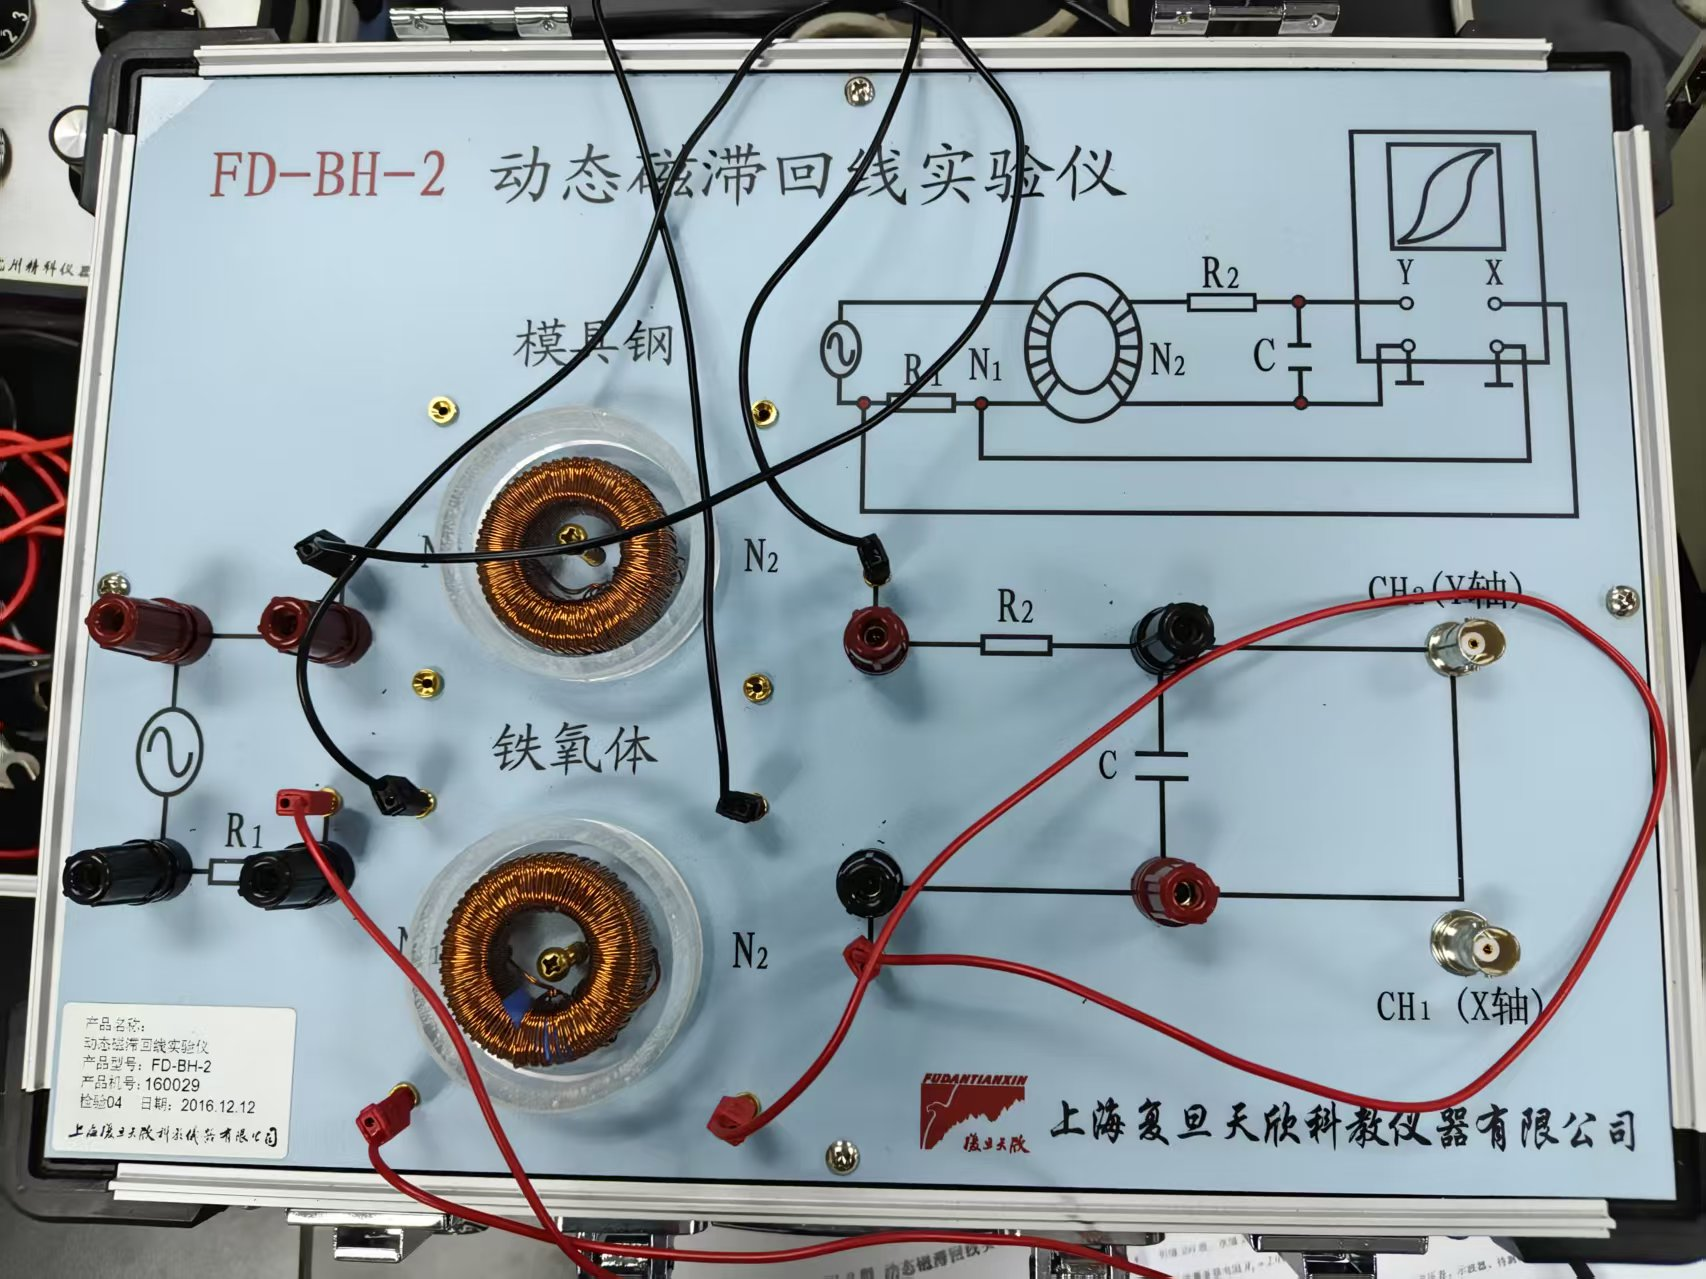
\includegraphics[width=\textwidth]{fig3a.jpg}
        \caption{实验电路模块}
    \end{subfigure}
    \hfil
    \begin{subfigure}[b]{0.3\textwidth}
        \centering
        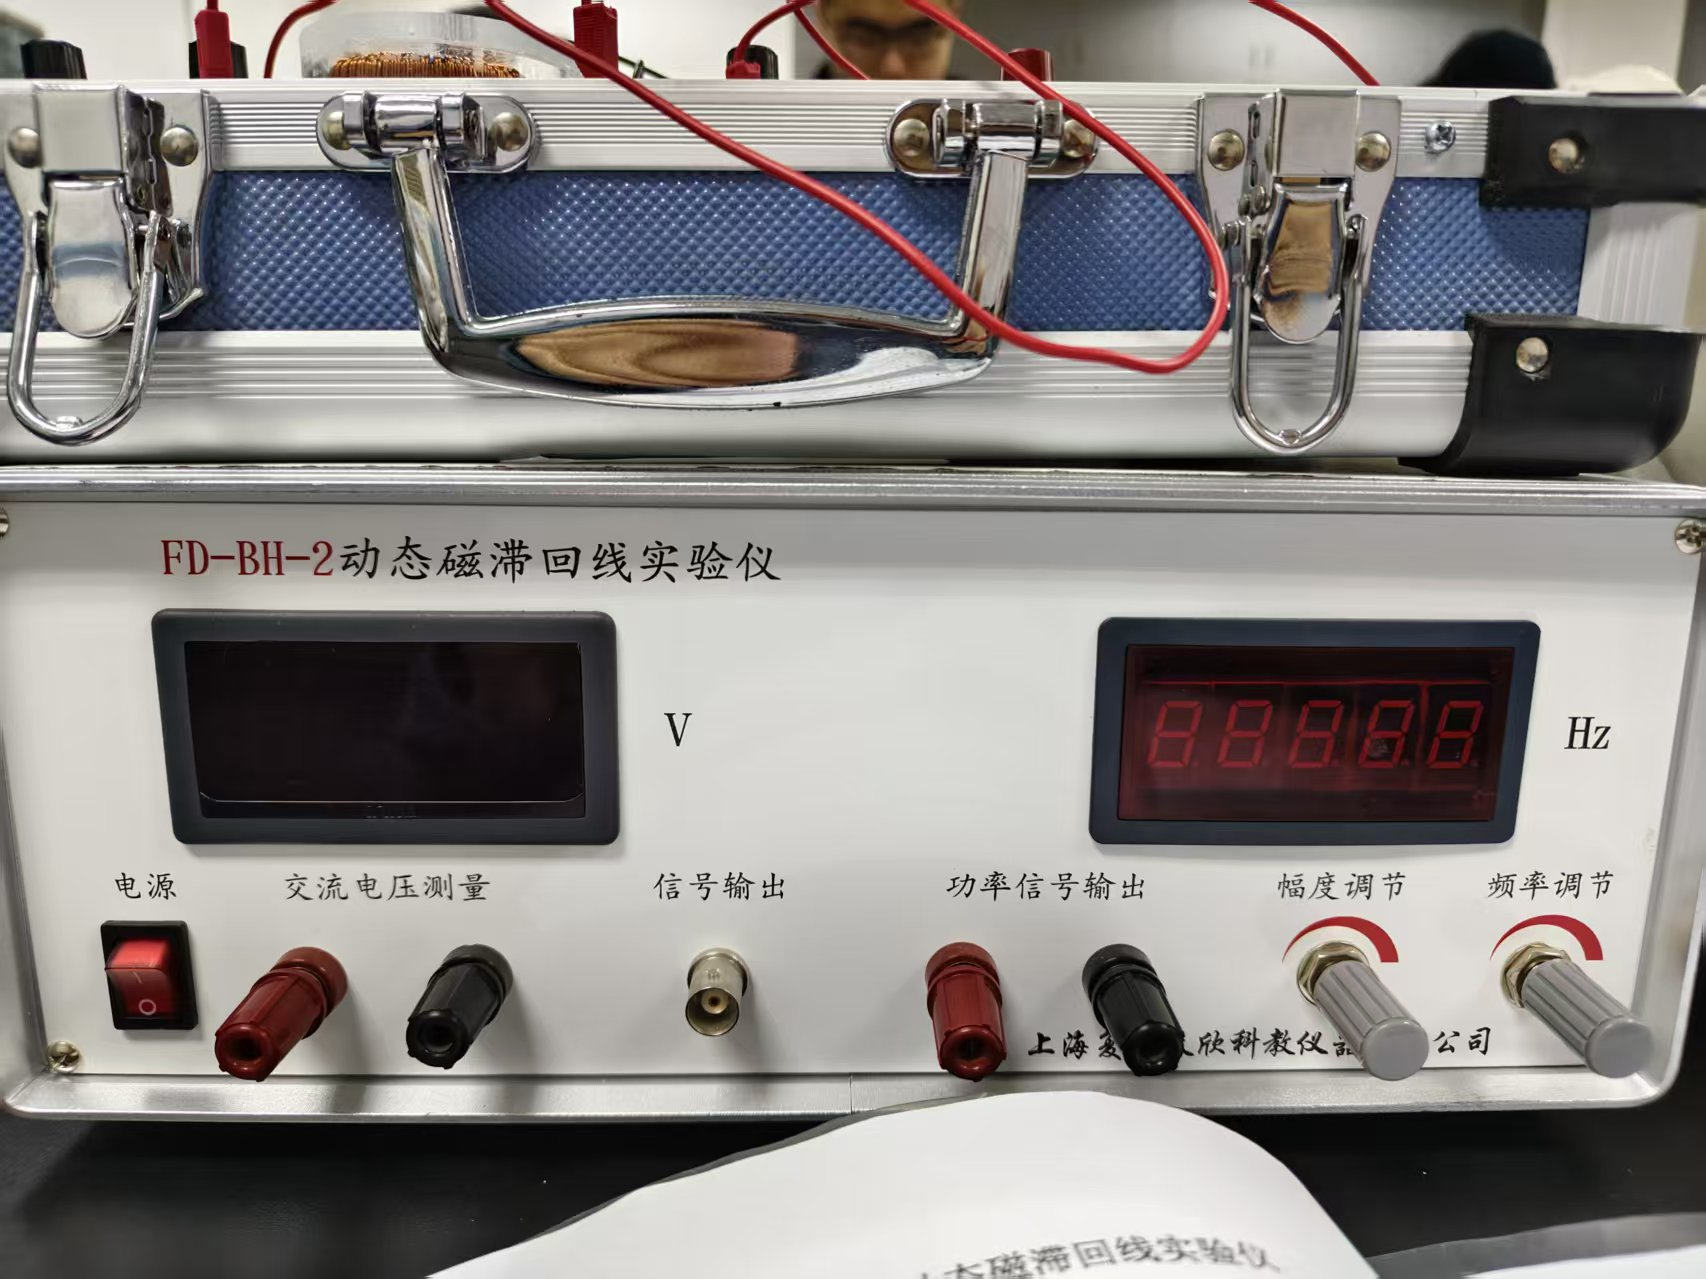
\includegraphics[width=\textwidth]{fig3b.jpg}
        \caption{正弦信号发生器}
    \end{subfigure}
    \hfil
    \begin{subfigure}[b]{0.3\textwidth}
        \centering
        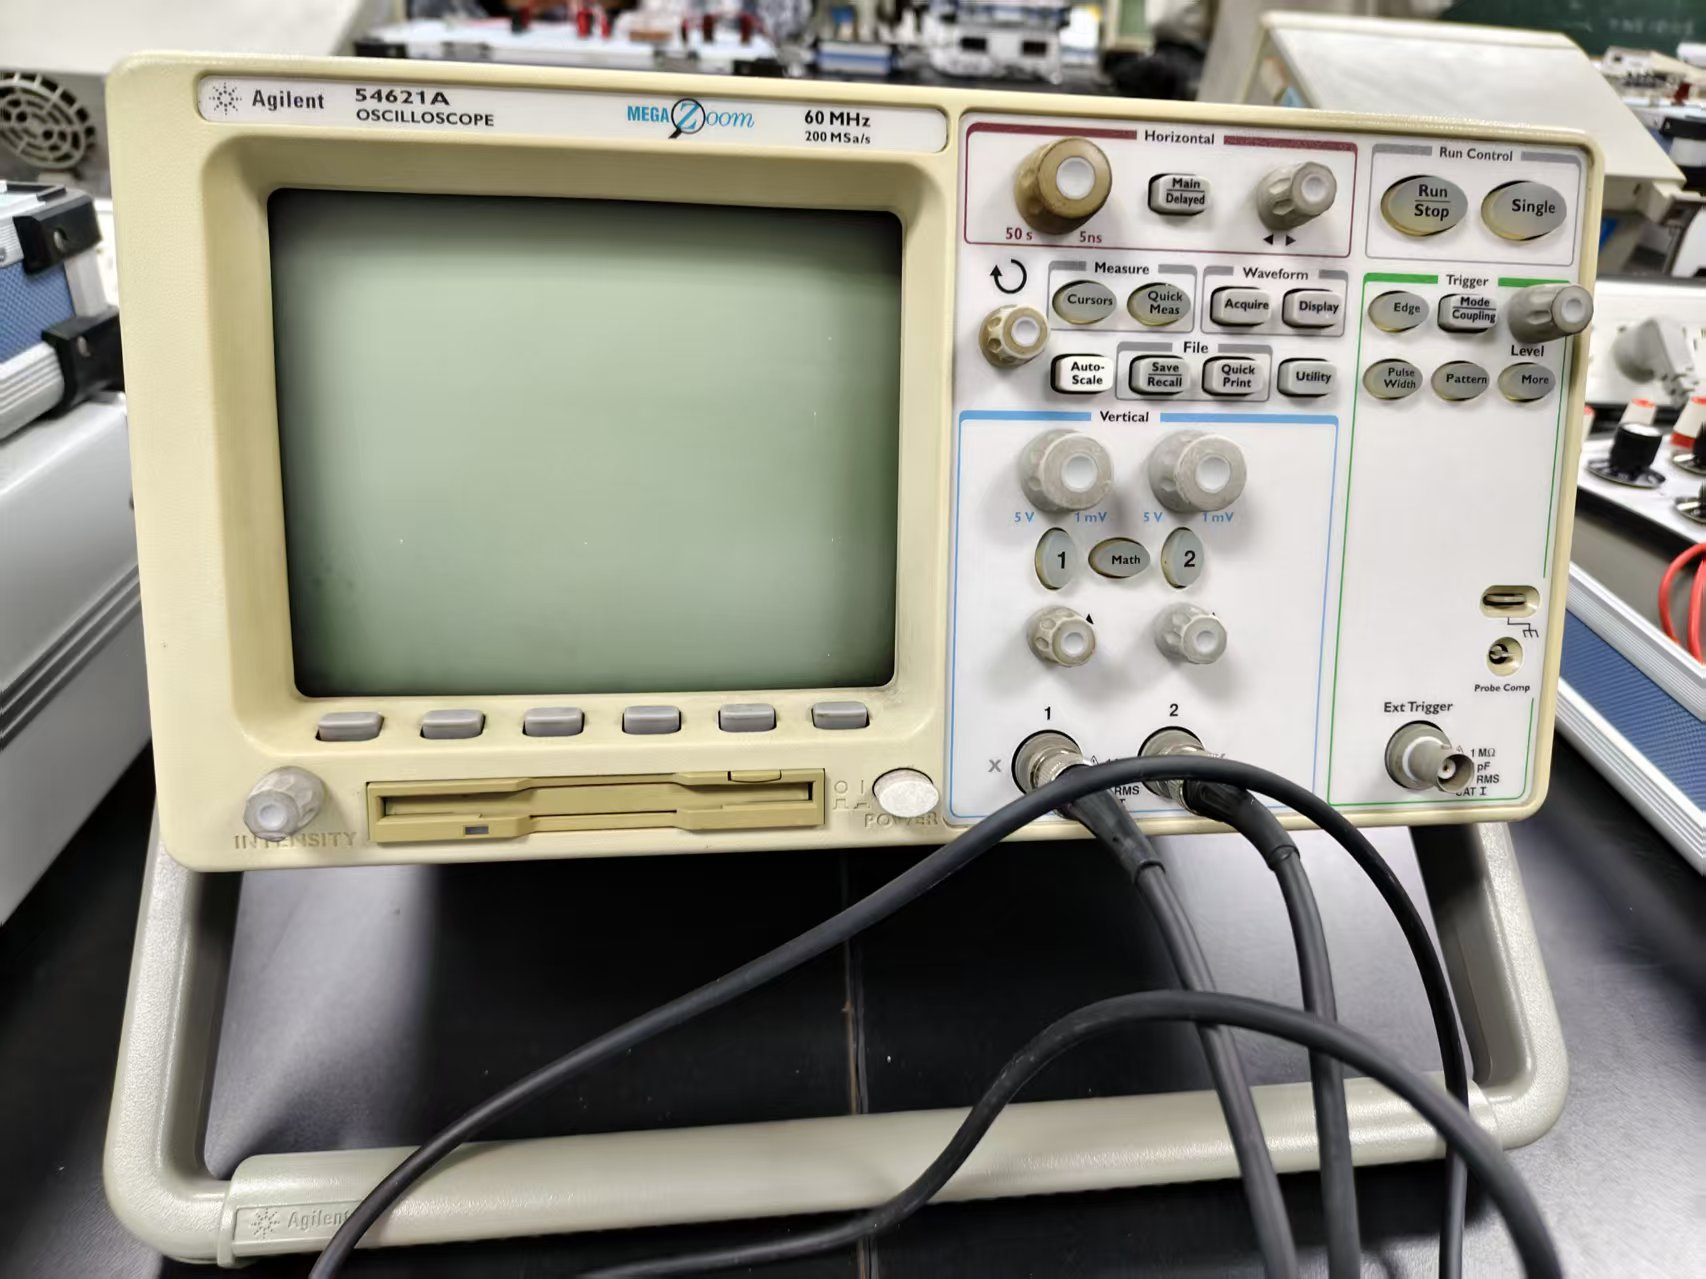
\includegraphics[width=\textwidth]{fig3c.jpg}
        \caption{示波器}
    \end{subfigure}
    \caption{实验仪器}
\end{figure}

本实验中:

（1）待测磁性样品:软磁铁氧体1只(环状)、初级 200 匝、次级 200 匝:硬磁模具钢(Cr12 合金钢)1只(环状).
初级 200 匝，次级 200 匝:两个样品内径 23.0mm、外径 38.0mm，高 10.0mm。计算得到 $l=119.38\, mm$ ， $S=1134.11\, mm^2$。

（2）初级线圈串联电阻 $R_1=2.0\, \Omega$，次级线圈电路串联电阻 $R_2=50.0\, K\Omega$，电容 $C=4.7\, \mu F$

\section{实验内容}
\subsection{观察和测量软磁铁氧体的动态磁滞回线}
1.按照 Figure 2 要求连接好电路图；

2.把示波器光点调至荧光屏中心。磁化电流从零开始，逐渐增大磁化电流，直至磁滞回线上的磁感应强
度 $B$ 达到饱和(即 $H$ 值达到足够高时，曲线有变平坦的趋势，这一状态属饱和)。磁化电流的频率 $f$ 取 $50\, Hz$ 左右。示波器的 $X$ 轴和 $Y$ 轴分度值调整至适当位置，使磁滞回线的 $B_m$ 和 $H_m$ 值尽可能充满整个荧光屏，
且图形为不失真的磁滞回线图形。

3.记录磁滞回线的顶点 $B_m$ 和 $H_m$ ，剩磁 $B_r$ ,和矫顽力 $H_c$ 。三个读数值(以长度为单位)，在作图纸上画出软磁铁氧体的近似磁滞回线。

4.测量软磁铁氧体的基本磁化曲线。现将磁化电流慢慢从大至小，退磁至零。从零开始，由小到大测量不同磁滞回线顶点的读数值 $B_i$ 和 $H_i$ ，用作图纸作铁氧体的基本磁化曲线（$B-H$ 关系）及磁导率与磁场强度关系曲线（$\mu-H$ 曲线），其中 $\mu=\frac BH$ 。

\subsection{观测硬磁 Cr12 模具钢（铬钢）材料的动态磁滞回线}
1.将样品换成 Cr12 模具钢硬磁材料，经退磁后，从零开始电流由小到大增加磁化电流，直至磁滞回线达到磁感应强度饱和状态。磁化电流频率约为 $f=50\, Hz$ 左右。调节 $X$ 轴和 $Y$ 轴分度值使磁滞回线为不失真图形。
注意硬磁材料交流磁滞回线与软磁材料有明显区别，硬磁材料在磁场强度较小时，交流滞回线为椭圆形回线，而达到饱和时为近似矩形图形，硬磁材料的直流滞回线和交流磁滞回线也有很大区别。

2.记录相应的 $B_m$ 和 $H_m$ ， $B_r$ 和 $H_c$ 值，在作图纸上近似画出硬磁材料在达到饱和状态使的交流磁滞回线。

\section{实验结果以及实验数据}

\subsection{饱和磁滞回线}
\begin{figure}[H]
    \centering
    
\includegraphics[width=0.5\textwidth]{fig4.jpg}
    \caption{软磁材料动态磁滞回线}
\end{figure}

\begin{table}[H]
    \centering
    \caption{$H_m$ 和 $B_m$，$B_r$ 和 $H_c$ 的测量结果}
    \vspace{2pt}
    \begin{tabular}{cccccccc}
        \hline \hline
        $2u_1/ \mathrm{mV}$     & $2u_2/ \mathrm{mV}$ & $2u_r/ \mathrm{mV}$ & $2u_c/ \mathrm{mV}$ &        $H_m/ \mathrm{A\cdot m^{-1}}$ & $B_m/ \mathrm{mT}$  & $B_r/ \mathrm{mT}$  & $H_c/ \mathrm{A\cdot m^{-1}}$     \\
        606.3                    & 37.2                 & 20.8                 & 54.7        &        253.94              & 19.27          & 10.77          & 22.91             \\
        \hline \hline
    \end{tabular}
\end{table}

\begin{figure}[H]
    \centering
    
\includegraphics[width=0.6\textwidth]{fig6.jpg}
    \caption{软磁铁氧体近似磁滞回线}
\end{figure}

\subsection{基本磁化曲线测量}
\begin{longtable}{c c c c c}
\caption{实验数据}\label{tab:data_vertical}\\
\hline\hline
$i$ & $2u_1$/mV & $2u_2$/mV & $H_i$/A$\cdot$m$^{-1}$ & $B_i$/mT \\
\hline
\endfirsthead

\hline
$i$ & $2u_1$/mV & $2u_2$/mV & $H_i$/A$\cdot$m$^{-1}$ & $B_i$/mT \\
\hline
\endhead

\hline\hline
\endfoot

\hline\hline
\endlastfoot

1  & 46.56  & 6.62 & 19.5007539  & 3.429341069 \\
2  & 53.28  & 7.81 & 22.31529569 & 4.045793618 \\
3  & 55.78  & 8.38 & 23.36237226 & 4.341069208 \\
4  & 57.66  & 8.94 & 24.14977383 & 4.631164525 \\
5  & 60.31  & 9.63 & 25.25967499 & 4.988603398 \\
6  & 64.06  & 10.30 & 26.83028983 & 5.335681724 \\
7  & 81.25  & 12.90 & 34.02998827 & 6.682552839 \\
8  & 94.69  & 14.20 & 39.65907187 & 7.355988396 \\
9  & 104.37 & 17.50 & 43.71335232 & 9.065478657 \\
10 & 123.44 & 20.30 & 51.70045234 & 10.51595524 \\
11 & 150.00 & 23.10 & 62.82459373 & 11.96643183 \\
12 & 170.00 & 25.20 & 71.20120623 & 13.05428927 \\
13 & 208.13 & 28.30 & 87.17121796 & 14.66017406 \\
14 & 257.80 & 30.90 & 107.9745351 & 16.00704517 \\
15 & 325.00 & 33.40 & 136.1199531 & 17.30211355 \\
16 & 426.60 & 35.50 & 178.6731446 & 18.38997099 \\
17 & 517.20 & 37.00 & 216.6191992 & 19.16701202 \\
18 & 606.30 & 37.50 & 253.9370079 & 19.42602569 \\
19 & 746.90 & 40.60 & 312.8245937 & 21.03191048 \\
20 & 928.10 & 41.90 & 388.7167030 & 21.70534604 \\

\end{longtable}


\begin{figure}[H]
    \centering
    
\includegraphics[width=0.9\textwidth]{Figure_1.png}
\end{figure}
\begin{figure}[H]
    \centering
    
\includegraphics[width=0.9\textwidth]{Figure_2.png}
\end{figure}

\subsection{硬磁 Cr12 模具钢材料的动态磁滞回线观测}
\begin{figure}[H]
    \centering
    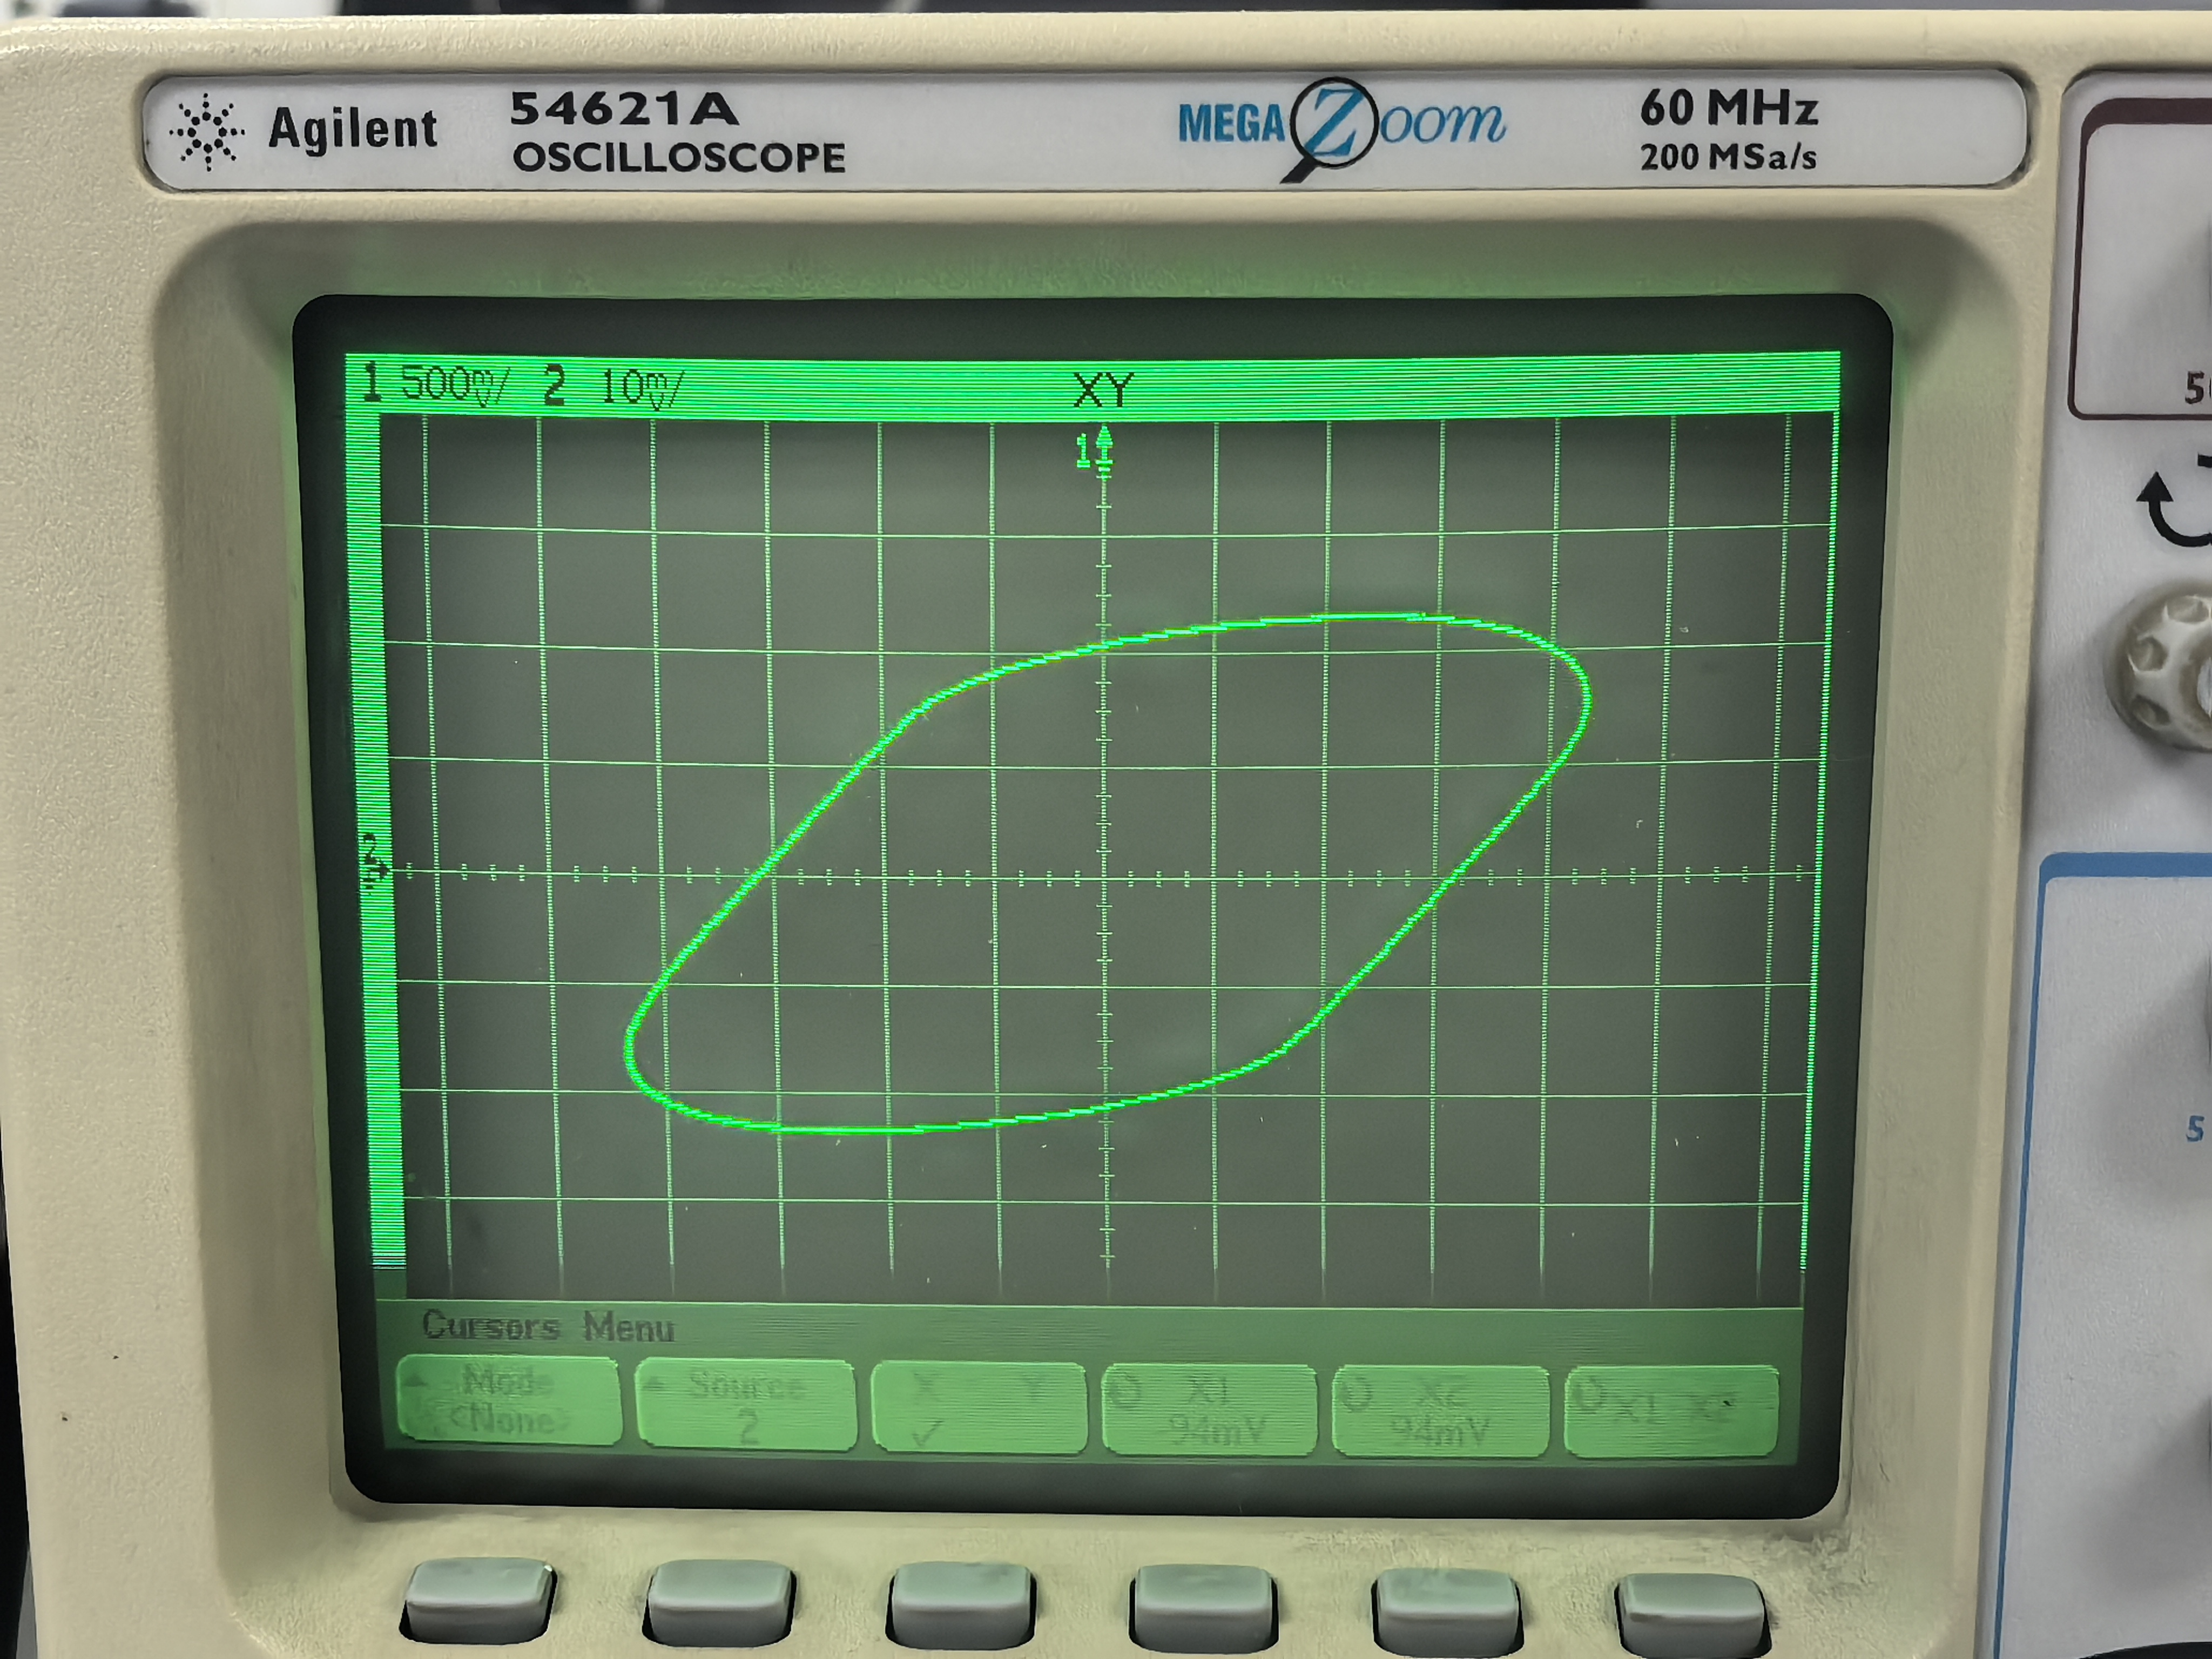
\includegraphics[width=0.5\textwidth]{fig5.jpg}
    \caption{硬磁材料动态磁滞回线}
\end{figure}

\begin{table}[H]
    \centering
    \caption{$H_m$ 和 $B_m$，$B_r$ 和 $H_c$ 的测量结果}
    \vspace{2pt}
    \begin{tabular}{cccccccc}
        \hline \hline
        $2u_1/ \mathrm{V}$     & $2u_2/ \mathrm{mV}$ & $2u_r/ \mathrm{mV}$ & $2u_c/ \mathrm{V}$ &        $H_m/ \mathrm{A\cdot m^{-1}}$ & $B_m/ \mathrm{mT}$  & $B_r/ \mathrm{mT}$  & $H_c/ \mathrm{A\cdot m^{-1}}$     \\
        4.25                    & 45.9                 &  32.8                &    3.8     &      1780.03              &  23.78          & 16.99          & 1591.56             \\
        \hline \hline
    \end{tabular}
\end{table}

\begin{figure}[H]
    \centering
    
\includegraphics[width=0.6\textwidth]{fig7.jpg}
    \caption{硬磁材料近似磁滞回线}
\end{figure}

\end{document}